\documentclass[29pt,a4paper]{moderncv}

% moderncv themes
%\moderncvtheme[blue]{casual}                 % optional argument are 'blue' (default), 'orange', 'red', 'green', 'grey' and 'roman' (for roman fonts, instead of sans serif fonts)
\moderncvtheme[green]{banking}                % idem

\usepackage[T1]{fontenc}
% character encoding
\usepackage[utf8x]{inputenc}               	% replace by the encoding you are using
\usepackage[italian]{babel}
\usepackage{color}

% adjust the page margins
\usepackage[scale=0.8]{geometry}
\recomputelengths                          	% required when changes are made to page layout lengths

\fancyfoot{} % clear all footer fields
\fancyfoot[L,RO]{\thepage}           		% page number in "outer" position of footer line
\fancyfoot[R,LO]{\footnotesize} 			% other info in 


\begin{document}

\section{\textbf{Change History:}}
\begin{tabbing}
\\\textbf{Date:} ~~~~~~~~~~~~~~~~~\= \textbf{Version Update:}~~~~~~~ \= \textbf{Member:}~~~~~~~~~~~~~~\= \textbf{Description:}\\
2013/08/22\> 1.0 \> fractals \> Document created.\\
2013/08/24 \> 1.1 \> fractals \> References Updated\\
2013/08/24 \> 1.2 \> fractals \> Outstanding Risks/Challenges added\\
2013/08/24 \> 1.3 \> fractals \> Support for Latex and Mimetex Libraries updated\\
2013/08/24 \> 1.4 \> fractals \> System Description updated\\
2013/08/24 \> 1.5 \> fractals \> Team Portfolio added. \\
2013/08/24 \> 1.6 \> fractals \> Responsibilities added for: Michelle Peens\\
2013/08/24 \> 1.7 \> fractals \> Responsibilities added for: Stephan Botha\\	
2013/08/24 \> 1.8 \> fractals \> Responsibilities added for: Janine Venter\\
2013/08/24 \> 1.9 \> fractals \> Issue Management Plan updated\\
2013/08/24 \> 2.0 \> fractals \> Software Development Process updated\\
2013/08/24 \> 2.1 \> fractals \> Project Progress updated\\
2013/08/24 \> 2.2 \> fractals \> Software Development Process updated\\
2013/08/24 \> 2.3 \> fractals \> Project Progress updated\\
2013/09/15 \> 2.4 \> Michelle Peens \> Kanban board created.\\
2013/09/15 \> 2.5 \>  Michelle Peens \> Kanban board updated\\
2013/09/15 \> 2.6 \> Stephan Botha \> Kanban board updated\\
2013/09/15 \> 2.7 \> Janine Venter \> Kanban board updated\\
2013/09/15 \> 2.8 \> Janine Venter \> Outstanding Risks/Challenges updated\\
2013/09/15 \> 2.9 \> Janine Venter \> Team Profiles updated\\
2013/09/15 \> 3.0 \>  Janine Venter \> Project Scope updated\\
2013/09/15 \> 3.1 \> Janine Venter \> System Description updated\\
2013/09/15 \> 3.2 \> Janine Venter \> Support for Latex and \\ \> \> \> Mimetex Libraries updated\\
2013/09/15 \> 3.3 \> Janine Venter \> Messaging updated\\
2013/09/23 \> 3.4 \> Michelle Peens \> Updated the Kanban board\\
2013/10/04 \> 3.5 \> Michelle Peens \> Updated Burndown Chart\\
2013/10/04 \> 3.6 \> Michelle Peens \> Added remaining outstanding challenges\\
2013/10/11 \> 3.7 \> Michelle Peens \> Updated the System Description\\
2013/10/11 \> 3.8 \> Michelle Peens \> Updated Burndown Chart\\
2013/10/12 \> 3.9 \> Janine Venter \> Updated the Kanban board\\
2013/10/12 \> 4.0 \> Janine Venter \> Updated Open Issues\\
2013/10/12 \> 4.1 \> Janine Venter \> Updated System Description\\


\end{tabbing}

\newpage
\section{\textbf{Table of Contents:}}
\begin{tabbing}
\\\textbf{Subject}: ~~~~~\= ~~~~~~~~~~~~~~~~~~~~~~~~~~~~~~~~~~~~~~~~~~~~~~~~~~~~~~~~~~~~~~~~~~~~~~~~~~~~~~~~~~~~~~~\= \textbf{Page}:
\\\newline
1. Introduction \> \> 3\\							
\> 1.1 Purpose 	\> 3\\							
\> 1.2 Document Conventions\> 3 					\\
\> 1.3 Project Scope \> 3							\\
\> 1.4 References \> 3							\\
2. System Description \> \> 4					\\
3. Software Development Process \> \> 5				\\
4. Team Profile\> \> 6 				\\
5. Issue Management Plan \> \> 7 	\\
6. Project Progress \> \> 8 	\\
\> 6.1 Kanban Board \> 9\\
\> 6.2 Burndown Chart \> 11\\
7. Outstanding Risks/Challenges \> \> 13 	\\
8. Open Issues \> \> 14 	\\
9. Glossary \> \> 15 	\\
\end{tabbing}

\newpage
	%\maketitle
	%\vspace{-10mm}
	%Section
	\section*{\textbf{1. Introduction}}
	\vspace{4mm}
	
		\textbf{1.1 Purpose}
			\\The purpose of this document is to provide our client with a high level overview of the architectural strategies or tactics and patterns that will form a basis for the development of the Latex Chat Application. The overall outline of these concepts and how they are implemented will provide our team with a means to achieve the given set of requirements as previously agreed upon in the Requirements and Design document.\\
		\vspace{1mm}
		
		\noindent \textbf{1.2 Document Conventions}
			\begin{itemize}
				\item Document Formatting: LaTeX
			\end{itemize}
		\vspace{5mm}
		%Section
		
		\noindent \textbf{1.3 Project Scope}
			\\The aim of the project is to develop an open source android XMPP chat client which supports the embedded LaTeX base equations which are rendered as images. LaTeX based equations will be rendered on the handset to produce mathematical equations. Our system will also provide the ability to view, edit and correct equations before sending.
			\parindent 5mm The application will provide a similar functionality to yaxim. Exchange of images and mathematical expressions will be possible through our software solution. The TeXchat application will have the ability to show a preview of the entered text send the equation as LaTeX code and then render it on the receiving end on the client handset.
		\vspace{5mm}
		
	\noindent \textbf{1.4 References}
		\begin{itemize}
		\item Mr. Will van Heerden.
		\end{itemize}
		\vspace{5mm}
		
	%Section
\newpage
\section*{\textbf{2. System Description}}
	\vspace{4mm}
		 The goal of our software application is to provide a chat service that will allow users to exchange normal text messages and send mathematical equations displayed in a rendered image format.  The application is intended to provide a service to users that require the ability and support for a chat client that allows them to communicate more efficiently and effortlessly in a scientific, and mathematical context. It will provide a more usable mobile version of a Latex chat application.\\ 
		
		\noindent\textbf{Support for LaTeX and MimeTeX Libraries} \\
		\parindent 5mm The application makes use of a Latex based library (MimeTeX) for the the rendering of equations as images on the mobile device.  For this reason we have implemented the support for the MimeTex library, through the use of the Android NDK (Native Development Kit), which allows us to embed the native C/C++ code of the MimeTeX library, in the source code. 
		\parindent 5mm The NDK acts as a bridge between the C/C++ code and Java code. The library is compiled through Eclipse using a special makefile that sets the correct compiler flags to indicate that it is in math mode and not text mode. The compiler flags represent different capabilities of the MimeTeX library, in this case we set it to math mode to support the mathematical LaTeX equations.\\
		
		
		\noindent\textbf{Messaging}
		\\parindent 5mm The purpose of this application is for messaging to be possible between multiple clients on the server. The application now supports this feature as well as allowing a user to send both plain text messages and Latex based equations, which are rendered on the client side and displayed as an inline images.\\
		The rendering of the Latex based equations on the client side is provided through the use of the Mimetex library. The messages sent between the various clients on the server is stored statically through making use of a client side SQLite database, which also provides the functionality for the retrieval of messages.
		\\Unsent messages, such as messages sent while the user was offline, is stored on the server and as soon as the client is online these messages are fetched and displayed on the user's handset. The server uses a queue to store these messages.\\
		
		\noindent\textbf{Login}
		\\The application allows a user to log in using an appropriate username and password combination. A user is authenticated by logging into the server.  If a username and password combination is invalid the server will automatically hinder the user from logging in. Our user authentication component is implemented by the functionality provided by the server. The user is informed by the application that his/her attempt to log in was unsuccessful.\\
		
		\noindent\textbf{Register}
		\\The application allows someone to register to the TexChat service as a new user. Through the user registration form the user provides the necessary information and selects a username and password combination that is later used to authenticate the user on the server. After a user is successfully registered, he can immediately log in and start using the messaging functionality provided.
		
	\vspace{5mm}
		
\newpage
	\section*{3. Software Development Process}
	\vspace{4mm}
	\\The process/methodology we are using throughout the development of our software solution for the Latex Chat Application will be a scaled down version of RUP, to accommodate our smaller group size, in conjunction with agile approaches, to accommodate the initial assumptions that the clients requirements for the application will change during the development of the application.
	
	This approach of combining the structured methods of RUP software development with agile approaches will allow us a structure for developing our software solution in an iterative manner, which will allow for changes, while still being able to design, code and test each version of its release in a controlled manner against the requirements set out for that specific release.
	
	Each release will have requirements, design, implementation, testing and integration phases, which are in line with the RUP process, and since this approach is based on regular and consistent user or client involvement, it will allow for changes in the requirements by the client during each release, which is in line with our agile approach.
	
	\vspace{5mm}

\newpage
	\section*{4. Team Profile}
	\noindent\textbf{Michelle Peens}
		\begin{itemize}
			\item Documentation
			\item Designing of the database
			\item Development of the system.
			\item Testing
			\item Project management
			\item Problem solving\\
		\end{itemize}
	
	\noindent\textbf{Stephan Botha}
		\begin{itemize}
			\item Documentation
			\item Development of the system
			\item Testing
			\item Project management
			\item Problem solving\\
		\end{itemize}
	
	\noindent\textbf{Janine Venter}
		\begin{itemize}
			\item Setting up meetings with the client and daily group meetings
			\item Documentation and converting documentation to LaTeX documentation.
			\item Testing
			\item Development of the system.
			\item Project management
			\item Problem solving
		\end{itemize}
\newpage
		\section*{Issue Management Plan}
		\begin{itemize}
			\item Issues are handled by discussing them with our client, as well as trying to resolve the issues by either working on it together or by doing research on the internet.
			\item All issues are resolved as quickly as possible except when it is a big hurdle. 
			\item All issues are discussed openly.
		\end{itemize}
		
\newpage
		\section*{6. Project Progress}
		During this release of our software solution we aimed to create the basis for further development phases.  This release is still in the initial phases of the overall development, and therefore only includes basic functionality as required for this release, namely:
		
		\begin{itemize}
			\item The application supports user login, and status update to ‘online’ on the server side.
			\item It allows the user to view messages that was previously sent, through making use of an SQLite database on the client side.
			\item The application has basic client chat support, in that it allows for sending basic text messages between clients on the server through the XMPP protocol.
			\item The Android NDK has also been included, so as to support the use of native code in the application.  This feature will be further developed in the next release to support the Mimetex libraries.	\\
		\end{itemize} \\
\newpage		
		\\ \noindent\textbf{6.1 Kanban Board} \\
  		\\	\begin{tabular}{| p{7cm} | p{7cm} | p{7cm} |}
				\hline
		    		\textbf{Tasks(To Do)} & \textbf{In Progress} & \textbf{Completed} \\ 
   				\hline
   				\hline
		    		Visual Aspects
		    		\begin{itemize}
			    		\item Display Of Messages.
			    		\item Display Of Various Pages.
		    		\end{itemize}
		    	 	& User Authentication. & User Login Component. \\ 
   				\hline
   				\hline
	   				User Profile Functionality:
	   				\begin{itemize}
	   					\item Profile Picture.
	   					\item Status Update.
	   					\item Online / Offline.
	   					\item General Information.
	   				\end{itemize}	
	   				& Unit Testing
	   				\begin{itemize}
	   					\item UI testing
		   				\item Services testing 
	   				\end {itemize}
	   				& SQLite Database\\
   				
				 Integration Testing & Integration Testing. & Android NDK\\
				
				\\ Exception Handling & Documentation & Including Mimetex Lib\\
				
				\\Adding/Deleting Contacts & Exception Handling & Image Rendering\\
				
				\\Integration Testing & Stability of Application & 
				Unit Testing
				\begin{itemize}
					\item Database Testing
				\end{itemize}
   				\\
   				
   				\\Test Usability &
   				Unit Testing 
   				\begin{itemize}
	   				\item UI Testing
	   				\item Services Testing 
   				\end{itemize} 
   				& Documentation\\
   				
   				\\Documentation & Visual Aspects & Exception Handling\\
   				
   				\\ & & Predefined Expression \\ & & Image Selections\\
				
				\\ & & Logo/Icon Design\\
				
				\\ & & Security Features \\ & &(Encryption)\\
				
				\\ & & Expr. String Handling\\
				
				\\ & & Settings Page\\
				
				\\ & & User Login Component\\
				
				\\ & & Contact List\\
				
				\\ & & Message Sending\\
				
				\\ & & Exit Component\\
			\end{tabular}
			
\newpage	
			\\	\begin{tabular}{| p{7cm} | p{7cm} | p{7cm} |}
				\hline
		    		\textbf{Tasks(To Do)} & \textbf{In Progress} & \textbf{Completed} \\ 
   				\hline			
				\\ & & SQLite Database \\ & & for Message Saving \\ & & User Details\\
				
				\\ & & Image Rendering \\ & & on Android Client\\
				
				\\ & & Documentation\\
				
				\\ & & Exception Handling\\
				
				\\ & & Testing Application \\ & & with Online Server\\
				
				\\ & & User Registration\\
				
				\\ & & Remember me \\& & Component\\
				
				\\ & & User Authentication\\
				
				\\ & & User Authorization\\
				
				\\ & & Database Cleanup\\
				
				\\ & & Adding and Deleting\\& & Contacts Component\\
				
				\\ & & Visual Aspects\\
				
				\\ & & Queueing of Messages\\ & & When Offline\\
   				
 			\end{tabular} \\
\newpage
		\noindent\textbf{6.2 Burndown Chart}
		\noindent\textbf{Progress Chart}
		\begin{figure*}
			\centering
			\\ 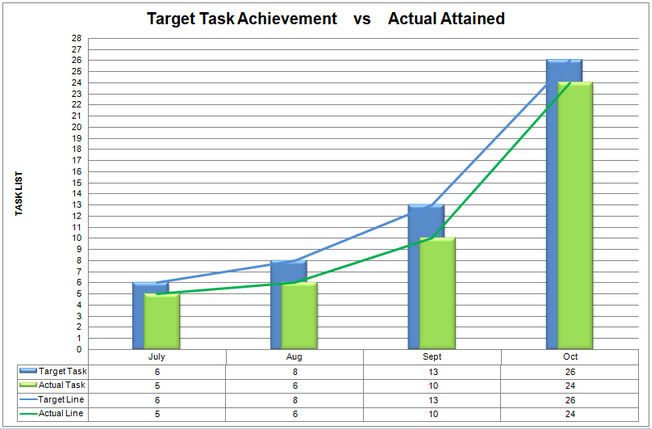
\includegraphics[width=6.0in, height=5.0in]{./chart.png}
			\\\caption{[Figure 1] Burndown Chart}
		\end{figure*}\\
		
\newpage
\begin{tabbing}
\\\textbf{Task:} ~~~~~~~~~~~~~~~~~~~~~~~~~~~~~~~~~~~~~~~~~~~~~~~~~~~~~\= \textbf{Task List:}\\

User Login Component \> 1\\
View Contact List	 \> 2 \\
Message Sending Component \> 3\\
Exit Component	\> 4 \\
SQLite Database	\> 5 \\
Android NDK	\> 6 \\
Mimetex Library	\> 7 \\
Image Rendering	\> 8 \\
String Handling\> 9 \\
Unit Testing	\> 10 \\
Integration Testing	\> 11 \\
Exception Handling\> 12 \\
Database Cleanup	\> 13 \\
User Registration	\> 14\\
User Authentication	\> 15 \\
Security Features	\> 16 \\
Settings Page\> 17 \\
Visual Aspects	\> 18 \\
Predefined Expression Images\> 19 \\
Adding / Deleting Contacts\> 20 \\
User Profile Functionality\> 21 \\
Logo / Icon Design\> 22 \\
Queuing of Messages\> 23 \\
Unit Testing	\> 24 \\
Integration Testing	\> 25 \\
Exception Handling	\> 26 \\

\end{tabbing}

\newpage
		\section*{7. Outstanding Risks/Challenges}
		\begin{itemize}
			\item The aesthetics of the application and overall user friendliness, although not the most important aspect, is still an outstanding challenge.
			\item Unit testing and Integration testing is limited as well.
		\end{itemize}
\newpage		
		\section*{8. Open Issues}
		Open Issues are only relevant towards the Android application itself, there are no open issues in terms of project management.\\
		Open Issues in the development of the application:
				\begin{itemize}
					\item Aesthetics of the application
					\item Usability
				\end{itemize}	
\newpage
		\section*{9. Glossary}
		\begin{itemize}
			\item Agile - Development methodology
			\item NDK - Native Development Kit
		\end{itemize}
\end{document}